\section{Ví dụ minh họa}
\label{sec:example}

\subsection{Ví dụ 1: CSDL cơ sở}

Xét cơ sở dữ liệu $D$ gồm 5 giao dịch trong Bảng \ref{tab:toy-db}. Nhóm chọn minsup tương đối $\theta = 0.6$, do đó minsup tuyệt đối là $\lceil 0.6 \times 5 \rceil = 3$.

\begin{table}[H]
    \centering
    \caption{CSDL toy dùng để minh hoạ FP-Max.}
    \label{tab:toy-db}
    \begin{tabular}{c c}
        \toprule
        Giao dịch & Item \\
        \midrule
        $T_1$ & $\{1,3,4\}$ \\
        $T_2$ & $\{2,3,5\}$ \\
        $T_3$ & $\{1,2,3,5\}$ \\
        $T_4$ & $\{2,5\}$ \\
        $T_5$ & $\{1,2,3,5\}$ \\
        \bottomrule
    \end{tabular}
\end{table}

Bước đầu tiên là đếm support của từng item. Kết quả là $\operatorname{sup}(1)=3$, $\operatorname{sup}(2)=4$, $\operatorname{sup}(3)=4$, $\operatorname{sup}(4)=1$, $\operatorname{sup}(5)=4$. Vì minsup tuyệt đối bằng 3, item $4$ bị loại. Để dựng FP-tree, các item còn lại trong mỗi giao dịch được sắp theo support giảm dần, nếu bằng nhau thì theo mã item tăng dần: $2 \prec 3 \prec 5 \prec 1$.

\begin{table}[H]
    \centering
    \caption{Các giao dịch sau bước tỉa và sắp thứ tự để dựng FP-tree.}
    \label{tab:toy-ordered}
    \begin{tabular}{c c c}
        \toprule
        Giao dịch & Sau khi loại item không phổ biến & Sau khi sắp theo thứ tự FP-tree \\
        \midrule
        $T_1$ & $\{1,3\}$ & $[3,1]$ \\
        $T_2$ & $\{2,3,5\}$ & $[2,3,5]$ \\
        $T_3$ & $\{1,2,3,5\}$ & $[2,3,5,1]$ \\
        $T_4$ & $\{2,5\}$ & $[2,5]$ \\
        $T_5$ & $\{1,2,3,5\}$ & $[2,3,5,1]$ \\
        \bottomrule
    \end{tabular}
\end{table}

Chèn tuần tự các giao dịch trong Bảng \ref{tab:toy-ordered} tạo ra FP-tree trong Hình \ref{fig:fptree-toy-ex}.

\begin{figure}[H]
    \centering
    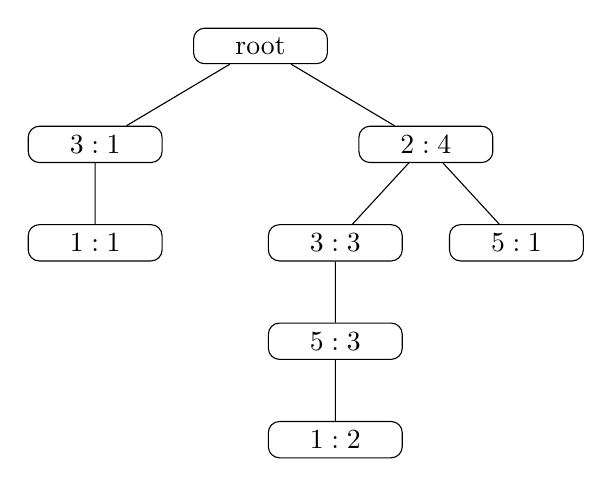
\begin{tikzpicture}[
        level distance=1.25cm,
        level 1/.style={sibling distance=4.2cm},
        level 2/.style={sibling distance=2.3cm},
        level 3/.style={sibling distance=1.8cm},
        every node/.style={draw, rounded corners, align=center, minimum width=1.7cm}
    ]
    \node {root}
        child { node {$3:1$}
            child { node {$1:1$} }
        }
        child { node {$2:4$}
            child { node {$3:3$}
                child { node {$5:3$}
                    child { node {$1:2$} }
                }
            }
            child { node {$5:1$} }
        };
    \end{tikzpicture}
    \caption{FP-tree cho CSDL toy Bảng \ref{tab:toy-db} sau bước tỉa và sắp thứ tự (Bảng \ref{tab:toy-ordered}).}
    \label{fig:fptree-toy-ex}
\end{figure}

Khác với FP-Growth, FP-Max duyệt header table theo thứ tự support \emph{tăng dần}, tức $1 \prec 2 \prec 3 \prec 5$ (item $1$ có support $3$, ba item còn lại có support $4$ nên xếp theo mã item). Bảng \ref{tab:toy-fpmax} ghi lại từng bước: head đang xét, conditional pattern base, tail (các item còn đủ support trong base), candidate tối đại sinh ra, và trạng thái danh sách MFI sau bước đó.

\begin{table}[H]
    \centering
    \caption{Vòng đệ quy FP-Max trên ví dụ cơ sở. Mỗi candidate được hợp nhất vào danh sách MFI theo quy tắc loại tập con nghiêm ngặt.}
    \label{tab:toy-fpmax}
    \small
    \begin{tabular}{c c c c c}
        \toprule
        Head & Conditional pattern base & Tail & Candidate & MFI sau bước \\
        \midrule
        $1$ & $(3):1,\ (2,3,5):2$ & $\{3\}$ & $\{1,3\}$ & $\{1,3\}$ \\
        $2$ & $\emptyset$ & $\emptyset$ & $\{2\}$ & $\{1,3\},\{2\}$ \\
        $3$ & $(2):3$ & $\{2\}$ & $\{2,3\}$ & $\{1,3\},\{2,3\}$ \\
        $5$ & $(2,3):3,\ (2):1$ & $\{2,3\}$ & $\{2,3,5\}$ & $\{1,3\},\{2,3,5\}$ \\
        \bottomrule
    \end{tabular}
\end{table}

Diễn giải các bước trong Bảng \ref{tab:toy-fpmax}. Khi xét head $\{1\}$, conditional pattern base gồm đường $(3)$ với count $1$ và đường $(2,3,5)$ với count $2$; chỉ item $3$ đạt support $3$ nên tail là $\{3\}$. Cây điều kiện co thành một đường, sinh candidate $\{1,3\}$ và khởi tạo MFI. Head $\{2\}$ có base rỗng (node $2$ nằm ngay dưới root) nên tạm thời cho candidate $\{2\}$. Đến head $\{3\}$, base $(2):3$ cho tail $\{2\}$ và candidate $\{2,3\}$; vì $\{2\}$ là tập con nghiêm ngặt của $\{2,3\}$ nên $\{2\}$ bị loại khỏi MFI. Cuối cùng head $\{5\}$ có base $(2,3):3$ và $(2):1$; tail $\{2,3\}$, cây điều kiện single-path cho candidate $\{2,3,5\}$, làm $\{2,3\}$ bị loại. Danh sách MFI hội tụ về hai phần tử.

Sau khi tính lại support trên $D$, tập kết quả của FP-Max là:
\[
    \{1,3\}:3, \qquad \{2,3,5\}:3.
\]

Để kiểm tra chéo thủ công, ta liệt kê toàn bộ tập phổ biến từ các item $\{1,2,3,5\}$: các đơn item $\{1\}:3,\{2\}:4,\{3\}:4,\{5\}:4$; các cặp $\{1,3\}:3,\{2,3\}:3,\{2,5\}:4,\{3,5\}:3$; và bộ ba $\{2,3,5\}:3$ (xuất hiện trong $T_2,T_3,T_5$). Trong chín tập phổ biến này, chỉ $\{1,3\}$ và $\{2,3,5\}$ là không có siêu tập phổ biến: mọi tập còn lại đều là tập con của một trong hai. Kết quả thủ công trùng khớp với đầu ra của FP-Max, và cũng đúng với cài đặt FPMax tham chiếu trong SPMF.

\subsection{Ví dụ 2: Tỉa theo siêu tập}

Trường hợp đặc biệt quan trọng của FP-Max là phép tỉa theo siêu tập: khi $head \cup tail$ đã nằm trong một MFI có sẵn, cả nhánh đệ quy bị cắt mà không cần dựng conditional FP-tree. Ví dụ này được thiết kế để phép tỉa thực sự kích hoạt.

Xét CSDL trong Bảng \ref{tab:prune-db} với $\theta = 0.5$, minsup tuyệt đối bằng 3.

\begin{table}[H]
    \centering
    \caption{CSDL thiết kế để kích hoạt phép tỉa theo siêu tập trong FP-Max.}
    \label{tab:prune-db}
    \begin{tabular}{c c}
        \toprule
        Giao dịch & Item \\
        \midrule
        $T_1$ & $\{a,b,c\}$ \\
        $T_2$ & $\{a,b,c\}$ \\
        $T_3$ & $\{a,b,c\}$ \\
        $T_4$ & $\{a,b,d\}$ \\
        $T_5$ & $\{a,b,d\}$ \\
        $T_6$ & $\{a,b,d\}$ \\
        \bottomrule
    \end{tabular}
\end{table}

Support của các item là $\operatorname{sup}(a)=6$, $\operatorname{sup}(b)=6$, $\operatorname{sup}(c)=3$, $\operatorname{sup}(d)=3$; tất cả đều đạt ngưỡng. Thứ tự dựng cây theo support giảm dần là $a,b,c,d$, cho FP-tree trong Hình \ref{fig:fptree-prune}.

\begin{figure}[H]
    \centering
    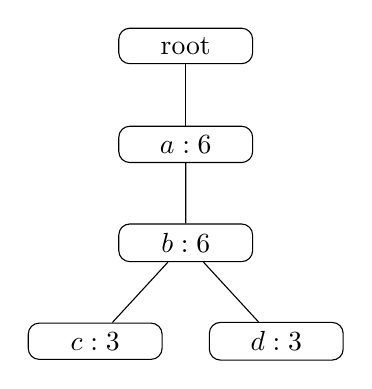
\begin{tikzpicture}[
        level distance=1.25cm,
        level 1/.style={sibling distance=3cm},
        level 2/.style={sibling distance=3cm},
        level 3/.style={sibling distance=2.3cm},
        every node/.style={draw, rounded corners, align=center, minimum width=1.7cm}
    ]
    \node {root}
        child { node {$a:6$}
            child { node {$b:6$}
                child { node {$c:3$} }
                child { node {$d:3$} }
            }
        };
    \end{tikzpicture}
    \caption{FP-tree cho CSDL Bảng \ref{tab:prune-db}. Node $b$ phân nhánh thành $c$ và $d$ nên cây không phải single-path.}
    \label{fig:fptree-prune}
\end{figure}

Vì node $b$ có hai con, cây không phải single-path nên thuật toán đi vào vòng đệ quy theo từng item. Header được duyệt theo support tăng dần: $c,d,a,b$ (hai item hiếm $c,d$ trước, hai item phổ biến $a,b$ sau). Bảng \ref{tab:prune-trace} ghi lại diễn biến.

\begin{table}[H]
    \centering
    \caption{Vòng đệ quy FP-Max trên CSDL Bảng \ref{tab:prune-db}. Hai item cuối bị tỉa nhờ kiểm tra siêu tập.}
    \label{tab:prune-trace}
    \small
    \begin{tabular}{c c c c l}
        \toprule
        Head & Conditional pattern base & $head\cup tail$ & Hành động & MFI sau bước \\
        \midrule
        $c$ & $(a,b):3$ & $\{a,b,c\}$ & dựng cây, candidate $\{a,b,c\}$ & $\{a,b,c\}$ \\
        $d$ & $(a,b):3$ & $\{a,b,d\}$ & dựng cây, candidate $\{a,b,d\}$ & $\{a,b,c\},\{a,b,d\}$ \\
        $a$ & $\emptyset$ & $\{a\}$ & $\{a\}\subseteq\{a,b,c\}$ $\Rightarrow$ tỉa & $\{a,b,c\},\{a,b,d\}$ \\
        $b$ & $(a):6$ & $\{a,b\}$ & $\{a,b\}\subseteq\{a,b,c\}$ $\Rightarrow$ tỉa & $\{a,b,c\},\{a,b,d\}$ \\
        \bottomrule
    \end{tabular}
\end{table}

Hai item hiếm $c$ và $d$ được xử lý trước, mỗi item có conditional pattern base $(a,b):3$ nên sinh hai tối đại $\{a,b,c\}$ và $\{a,b,d\}$. Khi đến item $b$, conditional pattern base là $(a):6$ cho tail $\{a\}$; vì $head \cup tail = \{a,b\}$ đã là tập con của MFI $\{a,b,c\}$, thuật toán cắt cả nhánh và \emph{không} dựng conditional FP-tree cho $b$ --- đây chính là chỗ tỉa tiết kiệm công sức. Item $a$ tương tự bị tỉa với $head\cup tail=\{a\}$. Tập kết quả là $\{a,b,c\}:3$ và $\{a,b,d\}:3$.

Trường hợp này làm rõ điểm khác biệt cốt lõi giữa FP-Max và FP-Growth. FP-Growth buộc phải xuất ra mọi tập phổ biến --- ở đây gồm $\{a\},\{b\},\{a,b\},\{a,c\},\{b,c\},\{a,b,c\},\dots$ với tổng cộng mười tập --- trong khi FP-Max chỉ giữ hai tối đại và bỏ qua phần lớn không gian nhờ phép tỉa. Cực điểm của hiệu ứng này là khi FP-tree co thành một đường đi dài $k$: FP-Growth sinh $2^k-1$ tập phổ biến, còn FP-Max nhận diện single-path và trả về đúng một tối đại; Ví dụ 3 minh hoạ cụ thể trường hợp đó. Đây là lý do FP-Max đặc biệt hiệu quả trên dữ liệu dày, nơi số tập phổ biến lớn theo cấp số mũ nhưng số tập tối đại nhỏ hơn nhiều.

\subsection{Ví dụ 3: FP-tree single-path}
\label{sec:example-singlepath}

Trường hợp đặc biệt thứ hai, và cũng là nguồn gốc của phần lớn hiệu năng FP-Max, là khi \emph{toàn bộ} FP-tree (hoặc một conditional FP-tree) co lại thành một đường đi duy nhất. Khi đó mọi item trên đường đều cùng xuất hiện trong các giao dịch sinh ra đường đó, nên hợp của chúng đã là một tập phổ biến; FP-Max nhận diện cấu trúc single-path và trả thẳng \emph{một} tối đại duy nhất mà không cần đệ quy qua từng head. Ví dụ này được thiết kế để chính cây gốc là single-path.

Xét CSDL trong Bảng \ref{tab:single-db} với $\theta = 0.5$, minsup tuyệt đối bằng 2.

\begin{table}[H]
    \centering
    \caption{CSDL thiết kế để FP-tree gốc co thành một đường đi duy nhất.}
    \label{tab:single-db}
    \begin{tabular}{c c}
        \toprule
        Giao dịch & Item \\
        \midrule
        $T_1$ & $\{a,b,c\}$ \\
        $T_2$ & $\{a,b,c\}$ \\
        $T_3$ & $\{a,b\}$ \\
        $T_4$ & $\{a\}$ \\
        \bottomrule
    \end{tabular}
\end{table}

Support của các item là $\operatorname{sup}(a)=4$, $\operatorname{sup}(b)=3$, $\operatorname{sup}(c)=2$; cả ba đều đạt ngưỡng. Mỗi giao dịch là tập con của giao dịch dài hơn (cấu trúc lồng nhau $\{a\}\subset\{a,b\}\subset\{a,b,c\}$), nên khi chèn theo thứ tự support giảm dần $a,b,c$, mọi giao dịch dùng chung tiền tố và FP-tree co thành một đường đi duy nhất trong Hình \ref{fig:fptree-single}.

\begin{figure}[H]
    \centering
    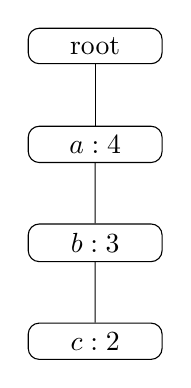
\begin{tikzpicture}[
        level distance=1.25cm,
        level 1/.style={sibling distance=3cm},
        every node/.style={draw, rounded corners, align=center, minimum width=1.7cm}
    ]
    \node {root}
        child { node {$a:4$}
            child { node {$b:3$}
                child { node {$c:2$} }
            }
        };
    \end{tikzpicture}
    \caption{FP-tree cho CSDL Bảng \ref{tab:single-db}. Không node nào phân nhánh nên cây là single-path, FP-Max trả thẳng một tối đại.}
    \label{fig:fptree-single}
\end{figure}

Vì root chỉ có một con và không node nào phân nhánh, thuật toán phát hiện single-path ngay tại lời gọi gốc. Thay vì duyệt header table và đệ quy theo từng head, FP-Max gom mọi item trên đường đạt minsup thành một candidate duy nhất $\{a,b,c\}$ với support bằng count nhỏ nhất trên đường ($\operatorname{sup}(c)=2$), rồi hợp vào danh sách MFI. Tập kết quả là:
\[
    \{a,b,c\}:2.
\]

Đối chiếu chi phí giữa hai thuật toán làm rõ giá trị của lối tắt single-path. Trên cùng CSDL này, FP-Growth phải liệt kê toàn bộ $2^3-1=7$ tập phổ biến trong Bảng \ref{tab:single-compare}; FP-Max chỉ giữ lại đúng tập tối đại bao trùm cả bảy. Khi đường dài $k$ thay vì $3$, khoảng cách này nới rộng thành $2^k-1$ so với $1$ --- đúng hành vi cấp số mũ đã nêu ở cuối Ví dụ 2.

\begin{table}[H]
    \centering
    \caption{So sánh đầu ra trên CSDL single-path Bảng \ref{tab:single-db}: FP-Growth liệt kê mọi tập con, FP-Max chỉ giữ tối đại.}
    \label{tab:single-compare}
    \begin{tabular}{l l}
        \toprule
        Thuật toán & Đầu ra \\
        \midrule
        FP-Growth & $\{a\}:4,\ \{b\}:3,\ \{c\}:2,\ \{a,b\}:3,\ \{a,c\}:2,\ \{b,c\}:2,\ \{a,b,c\}:2$ \\
        FP-Max & $\{a,b,c\}:2$ \\
        \bottomrule
    \end{tabular}
\end{table}
